\documentclass[italian]{article}
\usepackage[T1]{fontenc}
\usepackage[utf8]{inputenc}
\usepackage{lmodern}
\usepackage{hyperref}
\usepackage[a4paper,top=3cm,bottom=3cm,left=2.5cm,right=2.5cm]{geometry}
\usepackage[italian]{babel}
\usepackage{listings} %Per inserire codice
\usepackage[usenames]{color} %Per permettere la colorazione dei caratteri 
%Define the listing package
\usepackage{listings} %code highlighter
\usepackage{color} %use color
\usepackage{graphicx}
\graphicspath{ {./images/} }
\definecolor{mygreen}{rgb}{0,0.6,0}
\definecolor{mygray}{rgb}{0.5,0.5,0.5}
\definecolor{mymauve}{rgb}{0.58,0,0.82}

%Customize a bit the look
\lstset{ %
	backgroundcolor=\color{white}, % choose the background color; you must add \usepackage{color} or \usepackage{xcolor}
	basicstyle=\footnotesize, % the size of the fonts that are used for the code
	breakatwhitespace=false, % sets if automatic breaks should only happen at whitespace
	breaklines=true, % sets automatic line breaking
	captionpos=b, % sets the caption-position to bottom
	commentstyle=\color{mygreen}, % comment style
	deletekeywords={...}, % if you want to delete keywords from the given language
	escapeinside={\%*}{*)}, % if you want to add LaTeX within your code
	extendedchars=true, % lets you use non-ASCII characters; for 8-bits encodings only, does not work with UTF-8
	frame=single, % adds a frame around the code
	keepspaces=true, % keeps spaces in text, useful for keeping indentation of code (possibly needs columns=flexible)
	keywordstyle=\color{blue}, % keyword style
	% language=Octave, % the language of the code
	morekeywords={*,...}, % if you want to add more keywords to the set
	numbers=left, % where to put the line-numbers; possible values are (none, left, right)
	numbersep=5pt, % how far the line-numbers are from the code
	numberstyle=\tiny\color{mygray}, % the style that is used for the line-numbers
	rulecolor=\color{black}, % if not set, the frame-color may be changed on line-breaks within not-black text (e.g. comments (green here))
	showspaces=false, % show spaces everywhere adding particular underscores; it overrides 'showstringspaces'
	showstringspaces=false, % underline spaces within strings only
	showtabs=false, % show tabs within strings adding particular underscores
	stepnumber=1, % the step between two line-numbers. If it's 1, each line will be numbered
	stringstyle=\color{mymauve}, % string literal style
	tabsize=2, % sets default tabsize to 2 spaces
	title=\lstname % show the filename of files included with \lstinputlisting; also try caption instead of title
}
%END of listing package%

\definecolor{darkgray}{rgb}{.4,.4,.4}
\definecolor{purple}{rgb}{0.65, 0.12, 0.82}

%define Javascript language
\lstdefinelanguage{JavaScript}{
	keywords={typeof, new, true, false, catch, function, return, null, catch, switch, var, if, in, while, do, else, case, break},
	keywordstyle=\color{blue}\bfseries,
	ndkeywords={class, export, boolean, throw, implements, import, this},
	ndkeywordstyle=\color{darkgray}\bfseries,
	identifierstyle=\color{black},
	sensitive=false,
	comment=[l]{//},
	morecomment=[s]{/*}{*/},
	commentstyle=\color{purple}\ttfamily,
	stringstyle=\color{red}\ttfamily,
	morestring=[b]',
	morestring=[b]"
}

\lstset{
	language=JavaScript,
	extendedchars=true,
	basicstyle=\footnotesize\ttfamily,
	showstringspaces=false,
	showspaces=false,
	numbers=left,
	numberstyle=\footnotesize,
	numbersep=9pt,
	tabsize=2,
	breaklines=true,
	showtabs=false,
	captionpos=b
}
\author{
	Daniele Rigon - 857319 \\
}


\begin{document}
	
	\title{Tesi - Payment Request API}
	\maketitle
	
	\tableofcontents
	\pagebreak
	
	\section{Overview Payment Request}
	La PaymenteRequest API nasce con l'intento di creare esperienze di pagamento semplificate, in quanto ogni sito web ha il proprio sistema di pagamento e molti siti richiedono la ridigitazione manuale delle stesse informazioni più volte, le quali possono essere invece memorizzate e riutilizzate dall'API per completare più rapidamente le transazioni online.
	
	\subsection{Vantaggi}
	\begin{itemize}
	\item \textbf{Esperienza di acquisto rapida:} gli utenti immettono i propri dati una sola volta nel browser, e dopo averli inseriti non è più necessario reinserirli su siti diversi;
	\item \textbf{Esperienza coerente su ogni sito che supporta l'API:} poiché la pagina di pagamento è controllata dal browser si può personalizzare l'esperienza utente, ad esempio includendo la localizzazione per impostare automaticamente la lingua preferita dell'utente o altre features;
	\item \textbf{Gestione delle credenziali:} gli utenti possono gestire le loro carte di credito e gli indirizzi di spedizione direttamente nel browser. Un browser può anche sincronizzare queste "credenziali" tra dispositivi, rendendo più semplice per gli utenti passare dal desktop al cellulare e viceversa quando si acquistano oggetti;
	\item \textbf{Gestione coerente degli errori:} il browser può controllare la validità dei numeri delle carte e può comunicare all'utente se una carta è scaduta o sta per scadere, può suggerire automaticamente quale carta utilizzare in base ai modelli di utilizzo passati o alle restrizioni del commerciante, o consentire all'utente di dire quale sia la carta predefinita/preferita;
	\item \textbf{Esperienza utente migliorata:} meno tipizzazione, coerenza tra i siti Web, tra browser e sistemi operativi e nuove funzionalità del browser per semplificare il checkout, ecc;
	\item \textbf{Miglioramento della sicurezza:} la PaymentRequest API ha il potenziale per ridurre le opportunità di frode e può facilitare l'adozione di metodi di pagamento più sicuri. Purtroppo ci sono dei problemi di sicurezza analizzati al capitolo 4; 
	\item \textbf{Responsabilità inferiore:} in passato, per creare un'esperienza utente semplificata, i commercianti dovevano memorizzare le credenziali di pagamento degli utenti. Questo non è più necessario, il che può aiutare a ridurre la responsabilità del commerciante nei confronti del cliente.
	\end{itemize}
	
	\subsection{Come funziona}	
	La PaymentRequest API consente a un utente di completare una transazione più facilmente riutilizzando le informazioni memorizzate nel browser o in app di pagamento di terze parti.
	Quando l'utente preme un pulsante in una pagina di checkout collegata all'API il commerciante utilizza l'API per richiedere il pagamento. Il commerciante fornisce informazioni su prezzo, valuta e un elenco di metodi di pagamento accettati, e può inoltre richiedere al browser di creare un'interfaccia utente semplificata per raccogliere l'indirizzo di spedizione, le informazioni di contatto e altri elementi all'utente.
	Il browser determina quali metodi di pagamento sono supportati dal commerciante tra le varie "app di pagamento" mostrandole all'utente. 
	L'utente seleziona un'app di pagamento con la quale pagare, la quale può comportare ulteriori interazioni con l'utente (ad esempio per l'autenticazione). 
	Al completamento l'app di pagamento restituisce i dati tramite l'API al commerciante.

	\begin{figure}[h]
		\centering
		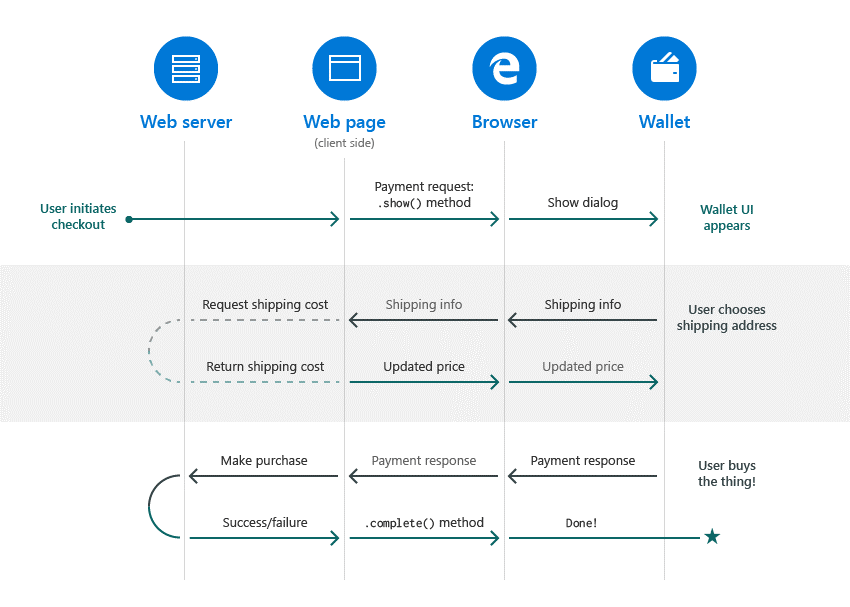
\includegraphics[width=1\linewidth]{SchemaPayment}
		\caption{Schema Payment Request API}
		\label{fig:Schema Payment}
	\end{figure}
	\pagebreak
	
	\subsection{Uso API}
	\subsubsection{Ruolo dell'utente}
	Gli utenti beneficiano del riutilizzo delle credenziali inserite nel browser o nelle app di pagamento. Quindi, quando si visita un sito Web che sfrutta la PaymentRequest API gli utenti avranno l'opportunità di sfruttare il riutilizzo semplificato delle credenziali archiviate.

	\subsubsection{Ruolo del commerciante}
	L'API influisce sul front end (l'interfaccia dell'esperienza utente) e non sul back-end, pertanto il commerciante non dovrebbe dover apportare modifiche all'elaborazione back-end dei vari metodi di pagamento; questo sarà compito del fornitore della pagina di pagamento il quale sostituirà i moduli Web con le chiamate alla PaymentRequest API.
	
	\subsubsection{Ruolo del browser}
	Il browser svolge diversi ruoli:
	\begin{itemize}
	\item Calcola l'intersezione dei metodi di pagamento accettati dal commerciante e registrati dall'utente;
	\item Visualizza l'interfaccia utente che consente all'utente di inserire le proprie informazioni;
	\item Funge da canale per i dati da e verso il commerciante e da e verso l'utente.
	\end{itemize}
	
	\subsubsection{Metodi di pagamento}
	La PaymentRequest API è progettata per funzionare con un gran numero di metodi di pagamento, i quali vengono identificati attraverso due strade:
	\begin{itemize}
		\item I metodi di pagamento definiti da W3C sono identificati come "basic-card" e sono composti da stringhe corte;
		\item I metodi di pagamento definiti da altre parti sono identificati dagli URL.
	\end{itemize}
	
	\subsubsection{App di pagamento}
	La PaymentRequest API, ovvero il browser, determina se un'app di pagamento "corrisponde" a una determinata transazione definendo un algoritmo che considera i metodi di pagamento accettati dal commerciante, dichiarati attraverso un elenco di identificativi del metodo di pagamento, passati attraverso l'API.
	Al fine di proteggere la privacy degli utenti i commercianti hanno accesso a informazioni molto limitate dell'utente. 
	
	Vediamo in che modo la PaymentRequest API influisce sul flusso dei metodi di pagamento che già supporta. Il normale flusso per gli utenti di solito implica qualcosa del genere:
	\begin{itemize}
	\item Scansione di un elenco di metodi di pagamento accettati;
	\item Scelta di un metodo;
	\item Per i metodi di pagamento che prevedono il lancio di un'app o la visita a un sito Web si invia l'utente a quell'app o sito;
	\item Pagamento completato.
	\end{itemize}
	La PaymentRequest API consente un flusso migliorato:
	\begin{itemize}
	\item L'utente preme un pulsante di acquisto singolo;
	\item Il browser visualizza le app di pagamento dell'utente che possono essere utilizzate per la transazione, ed è probabile che i browser supportino le preferenze dell'utente in modo che un'app di pagamento venga avviata automaticamente su un determinato sito Web, semplificando il checkout.
	\item Per i metodi di pagamento che prevedono il lancio di un'app o la visita a un sito Web, inviare l'utente a quell'app o sito; 
	\item Pagamento completato; 
	\end{itemize}
	
	
	\subsubsection{Differenze tra metodo di pagamento e app di pagamento}
	Un'app di pagamento è il software che l'utente utilizza per pagare, la quale può supportare uno o più metodi di pagamento e può essere implementata utilizzando diverse tecnologie. I browser possono anche fungere da app di pagamento, memorizzando le credenziali dell'utente. In generale più app di pagamento possono implementare lo stesso metodo di pagamento. 
	Vi sono casi importanti in cui è disponibile una sola app di pagamento autorizzata a supportare un metodo di pagamento, mentre ci sono casi in cui più app di pagamento possono servire diversi metodi di pagamento. In questo caso non è il commerciante che deve preoccuparsi dell'integrazione software, ma deve solamente richiedere le informazioni attraverso la PaymentRequest API.
	\pagebreak
	
	\section{Specifiche}
	\subsection{Metodi}
	Per utilizzare l'API lo sviluppatore deve fornire e tenere traccia di una serie di informazioni chiave, le quali vengono passate al costruttore PaymentRequest come argomenti e successivamente utilizzate per aggiornare la richiesta di pagamento visualizzata all'utente. Queste informazioni sono:
	\begin{itemize}
	\item \textbf{PaymentMethodData:} rappresenta i metodi di pagamento che il sito supporta;
	\item \textbf{PaymentDetails:} rappresenta i dettagli della transazione. Ciò include il costo totale e facoltativamente un elenco di beni o servizi acquistati, beni materiali, opzioni di spedizione o "modificatori" su come vengono effettuati i pagamenti: ad esempio "se paghi con una carta di credito di tipo X incorre in una tassa di elaborazione di tot";
	\item \textbf{PaymentOptions:} il PaymentOptions viene passato al costruttore PaymentRequest e fornisce informazioni sulla consegna del prodotto: ad esempio per i beni fisici il commerciante avrà bisogno di un indirizzo fisico dove spedire, mentre per i beni digitali e sufficeinte un'e-mail. Una volta che il PaymentRequest è stato costruito viene presentato all'utente finale tramite il metodo show(), il quale ritorna una promise che, una volta che l'utente conferma la richiesta di pagamento, si traduce in una PaymentResponse;
	\item \textbf{PaymentRequest:} la PaymentRequest serve a effettuare una richiesta di pagamento, in genere associata all'avvio di un processo di pagamento da parte dell'utente. La PaymentRequest consente agli sviluppatori di scambiare informazioni con l'user agent mentre l'utente sta fornendo dati in input. Poiché la visualizzazione simultanea di più interfacce PaymentRequest potrebbe confondere l'utente, questa specifica limita lo user agent a visualizzarne uno alla volta tramite il metodo show();
	\item \textbf{PaymentDetailsInit:} Il PaymentDetailsInit viene utilizzato nella costruzione della richiesta di pagamento;
	\item \textbf{PaymentResponse:} un PaymentResponse viene restituito quando un utente ha selezionato un metodo di pagamento e approvato una richiesta di pagamento.
	\end{itemize}

	\subsubsection{PaymentMethodData}
	PaymentMethodData contiene gli identificativi dei metodi di pagamento accettati dal sito Web e qualsiasi dato specifico del metodo di pagamento associato.
	\begin{lstlisting}
		const methodData = [
			{
				supportedMethods: "basic-card",
				data: {
					supportedNetworks: ["visa", "mastercard"],
					supportedTypes: ["debit", "credit"],
				},
			},
			{
				supportedMethods: "https://example.com/bobpay",
				data: {
					merchantIdentifier: "XXXX",
					bobPaySpecificField: true,
				},
			},
		];
	\end{lstlisting}
	
	\subsubsection{PaymentDetails}
	I details contengono informazioni sulla transazione che l'utente è invitato a completare.
	\begin{lstlisting}
		const details = {
			id: "super-store-order-123-12312",
			displayItems: [
			{
				label: "Sub-total",
				amount: { currency: "USD", value: "55.00" },
			},
			{
				label: "Sales Tax",
				amount: { currency: "USD", value: "5.00" },
				type: "tax"
			},
			],
			total: {
				label: "Total due",
				// The total is USD$65.00 here because we need to
				// add shipping (below). The selected shipping
				// costs USD$5.00.
				amount: { currency: "USD", value: "65.00" },
			},
		};
	\end{lstlisting}
	
	\textbf{Opzioni di spedizione}
	\\
	Qui vediamo un esempio di come aggiungere due opzioni di spedizione ai details.
	\begin{lstlisting}
		const shippingOptions = [
			{
				id: "standard",
				label: "Ground Shipping (2 days)",
				amount: { currency: "USD", value: "5.00" },
				selected: true,
			},
			{
				id: "drone",
				label: " Drone Express (2 hours)",
				amount: { currency: "USD", value: "25.00" }
			},
		];
		Object.assign(details, { shippingOptions });
	\end{lstlisting}
	
	\textbf{Modifiche condizionali alla richiesta di pagamento}
	\\
	Qui vediamo come aggiungere una tassa di elaborazione per l'utilizzo di una carta di credito. Si noti che richiede il ricalcolo del totale.
	\begin{lstlisting}
		// Credit card incurs a $3.00 processing fee.
		const creditCardFee = {
			label: "Credit card processing fee",
			amount: { currency: "USD", value: "3.00" },
		};
		
		// Modifiers apply when the user chooses to pay with
		// a credit card.
		const modifiers = [
			{
				additionalDisplayItems: [creditCardFee],
				supportedMethods: "basic-card",
				total: 
				{
					label: "Total due",
					amount: { currency: "USD", value: "68.00" },
				},
				data: 
				{
					supportedTypes: "credit",
				},
			},
		];
		Object.assign(details, { modifiers });
	\end{lstlisting}
	
	
	\subsubsection{PaymentOptions}
	Options contiene informazioni che lo sviluppatore ha bisogno dall'utente per eseguire il pagamento.
	\begin{lstlisting}
		const options = {
			requestPayerEmail: false,
			requestPayerName: true,
			requestPayerPhone: false,
			requestShipping: true,
		}
	\end{lstlisting}
	
	
	\subsubsection{PaymentRequest}
	Dopo aver raccolto tutti i bit di informazioni prerequisite, ora possiamo costruirne uno PaymentRequest e richiedere che il browser lo presenti all'utente.
	\begin{lstlisting}
		async function doPaymentRequest() 
		{
			try 
			{
				const request = new PaymentRequest(methodData, details, options);
				// See below for a detailed example of handling these events
				request.onshippingaddresschange = ev => ev.updateWith(details);
				request.onshippingoptionchange = ev => ev.updateWith(details);
				const response = await request.show();
				await validateResponse(response);
			} catch (err) 
				{
					// AbortError, SecurityError
					console.error(err);
				}
		}
		async function validateResponse(response) 
		{
			try {
				if (await checkAllValuesAreGood(response)) 
				{
					await response.complete("success");
				} 
				else {
					await response.complete("fail");
				}
			} catch (err) 
				{
					// Something went wrong...
					await response.complete("fail");
				}
		}
		doPaymentRequest();
	\end{lstlisting}
	
	\section{Rischi e sicurezza}
	La PaymentRequest API aumenta la sicurezza poichè:
	\begin{itemize}
		\item I commercianti possono ottenere un checkout semplificato senza memorizzare le credenziali dell'utente, in quanto lo fa l'API, rendendo i commercianti meno vulnerabili agli attacchi;
		\item La PaymentRequest API dovrebbe facilitare l'introduzione di metodi di pagamento più sicuri sul Web, come i pagamenti con carta tokenizzata;
		\item I proprietari dei metodi di pagamento disporranno di meccanismi standard per autorizzare software specifici a implementare il loro metodo di pagamento, che il browser può verificare attraverso una firma digitale.
	\end{itemize}
	I browser utilizzano una varietà di meccanismi per archiviare informazioni sensibili dell'utente, e attualmente W3C sta sviluppando nuove tecnologie per aumentarne la sicurezza.
	Per quanto riguarda la memorizzazione delle informazioni delle app di pagamento in modo sicuro, questo è un dettaglio di implementazione che è diverso per ogni app di pagamento, e tale sicurezza è a carico del provider dell'app di pagamento.
	
	\subsection{Esempio di un possibile attacco}
	\subsubsection{Descrizione dell'attacco}
	La sicurezza di usare la PaymentRequest API è che utilizza la gestione delle credenziali del browser che stiamo usando: se stiamo usando Chrome userà la gestione delle credenziali di Google, mentre se stiamo usando Edge userà Microsoft Pay (Nota: in questo caso è necessario anche autenticarsi con l'account Microsoft).
	Sicuramente il livello di sicurezza è elevato ma non è immune ad un attacco XSS, che potrebbe attaccare similmente al Phishing. 
	L'API apre una finestra dove inserire le credenziali, sicura perchè non vengono scritte nel DOM. Con un attacco XSS, alla chiamata dell'API, invece di questa finestra potrebbe venirne aperta un'altra uguale a quella originale, gestita però dall'attaccante. Essendo identica la vittima sarà convinta di inserire le credenziali in un posto sicuro, mentre invece saranno inviate all'attaccante invece di essere salvate nel browser tramite l'API.
	Sara possibile essere vittima di questo attacco solamente la prima volta che saranno inserite le credenziali in quanto l'API chiede l'inserimento delle credenziali solamente la prima volta, dopo saranno salvate e non verra piu chiesto l'inserimento da parte dell'utente.
	Sia su Chrome che su Microsoft l'inserimento del codice CVV viene chiesto in una pagina successiva, dopo aver inserito tutte le credenziali e averle salvate nella pagina corrente. Un attaccante, per essere sicuro di ottenere anche quel codice potrebbe inserire il form nella prima pagina cosicchè l'utente ignaro, inviando le informazioni, manda tutte quelle utili all'attaccante.
	\subsubsection{Come difendersi}
	Vi sono diverse metodologie per difendersi da questi tipi di attacchi:
	\begin{itemize}
	\item Una strategia per combattere il phishing è sicuramente quella di istruire le persone a riconoscere gli attacchi e ad affrontarli;
	\item Dato che il piu delle volte non e facile riconoscere questi attacchi, ci sono anche delle misure anti-phishing implementate nei browsers, come estensioni o toolbar, oltre a diversi software contro il phishing;
	\item Inoltre, la maggior parte dei siti bersaglio del phishing sono protetti da SSL con una forte crittografia, dove l'URL del sito web è usata come identificativo. Questo dovrebbe in teoria confermare l'autenticità del sito, ma nella pratica è facile da aggirare, sfruttando la vurnerabilita che sta nella user interface (UI) del browser. Nell'url del browser viene poi indicata la connessione utilizzara con diversi colori (blocco verde per certificato EV, scritta https in verde, ecc.).
	\end{itemize}

	\section{Implementazione PaymentRequest API su una pagina d'esempio}
	\subsection{Costruttore}
	L'oggetto PaymentRequest è costruito passando i seguenti parametri:
	\begin{itemize}
	\item \textbf{methodData:} una serie di identificativi del metodo di pagamento e tutti i dati pertinenti. Un identificativo del metodo di pagamento è una stringa che identifica un metodo di pagamento supportato;
	\item \textbf{details:} contiene le informazioni sulla transazione, come gli elementi pubblicitari in un ordine;
	\item \textbf{options:} contiene informazioni aggiuntive che il Wallet potrebbe dover raccogliere.
	\end{itemize}

	Nel seguente esempio stiamo consentendo agli utenti di pagare con qualsiasi carta di debito o di credito appartenente alle reti Visa, MasterCard o Amex. L'oggetto details contiene l'importo totale parziale, l'imposta sulle vendite e il totale dovuto; questi dettagli verranno mostrati all'utente nel portafoglio. Bisogna tenere presente che l'API non aggiunge elementi o calcola l'imposta sulle vendite, spetta al commerciante fornire le informazioni corrette. In questo esempio, stiamo vendendo un bene fisico, quindi chiediamo l'indirizzo di spedizione del cliente.

	\begin{lstlisting}
		var methodData = [
			{     
				supportedMethods: ['basic-card'],     
				data: {          
					supportedNetworks: ['visa', 'mastercard', 'amex'],
					supportedTypes: ['credit']                 
				}    
			}     
		];
		var details =  {
			displayItems: [
				{
					label: "Sub-total",
					amount: { currency: "USD", value : "100.00" } // US$100.00
				},
				{
					label: "Sales Tax",
					amount: { currency: "USD", value : "9.00" } // US$9.00
				}
			],
			total:  {
				label: "Total due",
				amount: { currency: "USD", value : "109.00" } // US$109.00
			}
		};	
		var options = {
			requestShipping: true 
		};
		var payment = new PaymentRequest(methodData, details, options);
	\end{lstlisting}
	
	\subsection{Visualizzazione dell'interfaccia utente, elaborazione del pagamento e visualizzazione dei risultati}
	Una volta creato l'oggetto PaymentRequest è possibile attivare il browser per visualizzare il wallet con request.show(). 
	\begin{figure}[h]
		\centering
		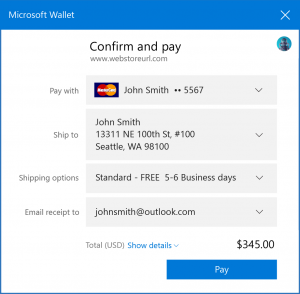
\includegraphics[width=1\linewidth]{wallet1}
		\caption{Wallet dopo la chiamata request.show()}
		\label{fig: Wallet dopo la chiamata request.show()}
	\end{figure}
	\pagebreak
	\\
	I clienti possono  selezionare le informazioni di pagamento, l'indirizzo di spedizione e altri campi appropriati e cliccare su Paga quando è pronto. A questo punto, gli utenti dovranno verificare la loro identità: in caso di esito positivo verrà soddisfatta la promise request.show() e verranno restituite al sito Web tutte le informazioni che il cliente ha fornito. Per il metodo di pagamento con carta di base l'oggetto risultante conterrà il nome del titolare della carta, il numero della carta, il mese di scadenza e altri campi pertinenti. Il commerciante può quindi utilizzare queste informazioni per elaborare la transazione sul back-end.
	Dopo che la risposta è tornata dal server, è possibile utilizzare result.complete('success') per visualizzare la schermata di successo o result.complete('fail') per indicare una transazione fallita.
	\pagebreak
	\begin{lstlisting}
	// Mostra l'interfaccia utente nativa
	payment.show()
	// Quando la promessa e soddisfatta, passa i risultati al tuo server per l'elaborazione
	.then(result => {
		return process(result).then(response => {
			if (response.status === 200) {
				// Mostra che la transazione ha avuto successo nell'interfaccia utente
				return result.complete('success');
			} else {
					// Mostra nell'interfaccia utente nativa che la transazione ha avuto esito negativo
					return result.complete('fail');
				}
			}).catch((err) => {
			console.error('User rejected request', err.message)
		}); 
	});
	\end{lstlisting}
	\pagebreak
	\begin{figure}[h]
		\centering
		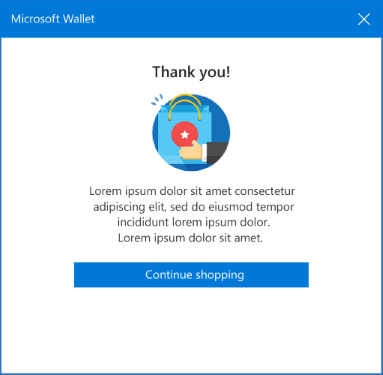
\includegraphics[width=1\linewidth]{wallet2}
		\caption{Wallet in caso di successo}
		\label{fig: Wallet in caso di successo}
	\end{figure}
	\begin{figure}[h]
		\centering
		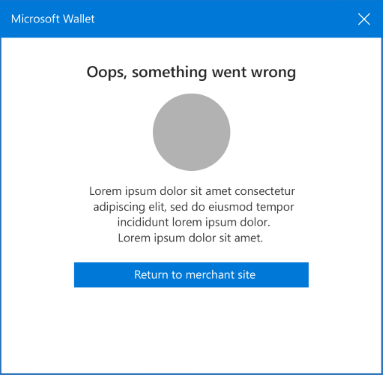
\includegraphics[width=1\linewidth]{wallet3}
		\caption{Wallet in caso di fail}
		\label{fig: Wallet in caso di fail}
	\end{figure}
	\pagebreak
	
	\subsection{Ascoltare gli eventi}
	Il prezzo potrebbe cambiare in base all'indirizzo di spedizione e alle opzioni di spedizione selezionate dal cliente. È possibile ascoltare tali modifiche con gli eventi shippingaddresschange e shippingoptionchange per ricalcolare di conseguenza i prezzi.
	\begin{lstlisting}
		payment.addEventListener("shippingaddresschange", function (changeEvent) {
			    // Elabora la modifica dell'indirizzo di spedizione
		});
		
		payment.addEventListener("shippingoptionchange", function (changeEvent) {
			// Modifica delle opzioni di spedizione del processo (ad esempio "spedizione in giornata")
		});
	\end{lstlisting}
	\pagebreak
	
	\section{Compatibilità web}
	\begin{figure}[h]
		\centering
		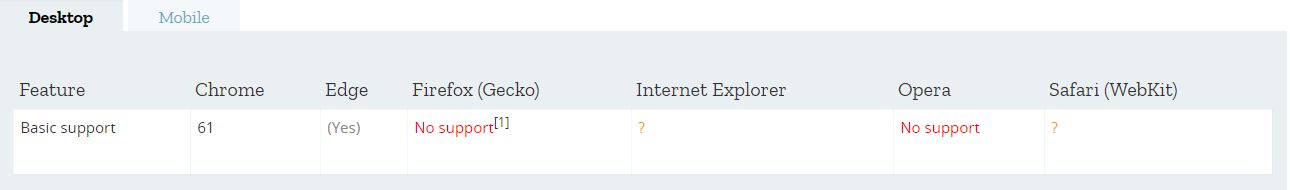
\includegraphics[width=1\linewidth]{Compatibilita1}
		\caption{Compatibilità desktop}
		\label{fig: Compatibilità desktop}
	\end{figure}
	\begin{figure}[h]
		\centering
		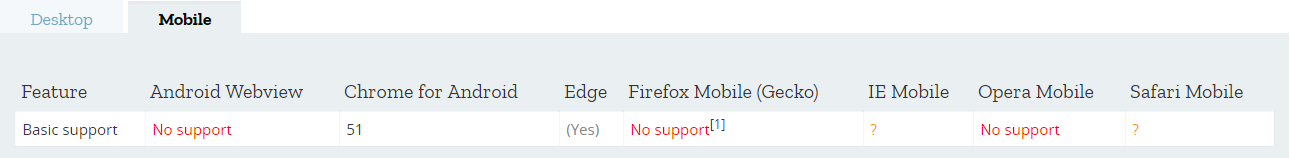
\includegraphics[width=1\linewidth]{Compatibilita2}
		\caption{Compatibilità mobile}
		\label{fig: Compatibilità mobile}
	\end{figure}

	\section{Conclusioni}
	La PaymentRequest API è uno potente strumento per migliorare l'esperienza utente sul Web offrendo ai clienti un'esperienza di acquisto più piacevole, pur avendo delle vulnerabilità difficili da rompere ma dalle quali ci si puo difendere.
\end{document}